\documentclass{article}

\usepackage[utf8x]{inputenc}
\usepackage[english,russian]{babel}
\usepackage{cmap}
\usepackage{graphicx}
\usepackage{float}
\graphicspath{ {./images/} }

\begin{document}

\begin{titlepage}
	\newpage
    \begin{center}
    {\bfseries САНКТ-ПЕТЕРБУРГСКИЙ ПОЛИТЕХНИЧЕСКИЙ УНИВЕРСИТЕТ ПЕТРА ВЕЛИКОГО}
  
	\noindent\makebox[\linewidth]{\rule{\textwidth}{0.4pt}} 

	\vspace{1cm}
	
	Институт компьютерных наук и технологий
	\\
	Высшая школа интеллектуальных систем и суперкомпьютерных технологий


  	\vspace{2cm}
  	
  	Отчет \\
    
  	По лабораторной работе №12 \\
  	\vspace{1em}
  	GNU Radio: Single Sideband transceiver
    
    \vspace{6em}
    
   \end{center}
   
   \vspace{3cm}

   \begin{flushright}
   
	Выполнил: \\
	Студент Соколов Д.С. \\ 
    Группа: 3530901 / 00203 
    
    \vspace{1em}
    
    Проверил: \\
    Преподаватель: Богач Н.В.
   
   \end{flushright}
   
   \vfill
   \begin{center}
   2023   
   \end{center}
	   
   
\end{titlepage}

\tableofcontents


\newpage
\section*{Введение}
\addcontentsline{toc}{section}{\protect\numberline{}Введение}

В данной лабораторной работе выполняется симуляция на примере однополосного приемопередатчика. В симуляцию включаются аппаратные составляющие компьютера - микрофон и динамики. Выполнение работы производится с GNU Radio 3.7+. Для создания графов соединений используется GUI gnuradio-companion (GRC).

\newpage
\section{Ход работы}
Создадим описания графов SSB receiver и SSB transmitter.

\subsection{SSB receiver}
Для начала загрузим тестовый файл \verb|ssb_lsb_256k_complex2.dat| и поместим в директорию с проектом.\\
Используя GRC создадим описание однополосного приемника, при этом задав необходимые значения переменным и выполнив конфигурацию блоков.

\vspace{1cm}
\begin{figure}[H]
\centering
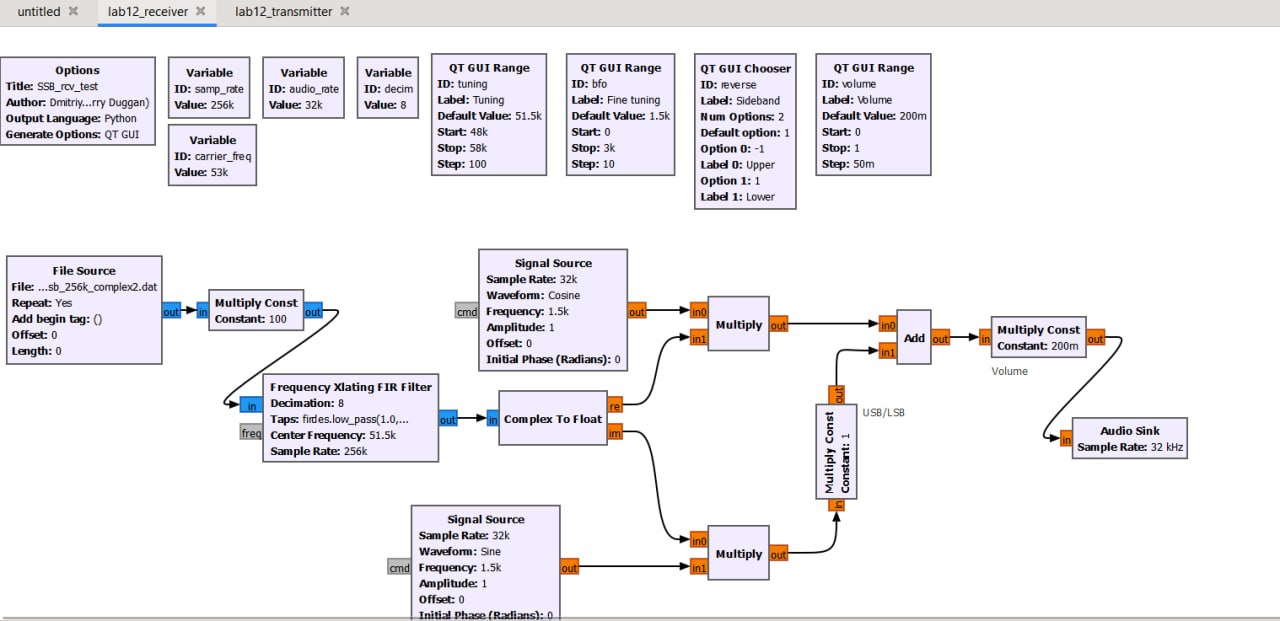
\includegraphics[width=\textwidth]{ssb_receiver_flowgraph.jpg}
\caption{SSB receiver flowgraph}
\end{figure}

Для тестирования приемника сгенерируем и запустим сгенерированный \texttt{.py} файл.\\
В открывшемся GUI окне можем управлять громкостью, sideband, tuning.
\\Изменим описание File source на ZMQ PULL Source, задав адресс подключения - \verb|tcp://127.0.0.1:50301| для объединения с transmitter.

\subsection{SSB transmitter}
С помощью GRC создадим описание однополосного передатчика.
\vspace{1cm}

\begin{figure}[H]
\centering
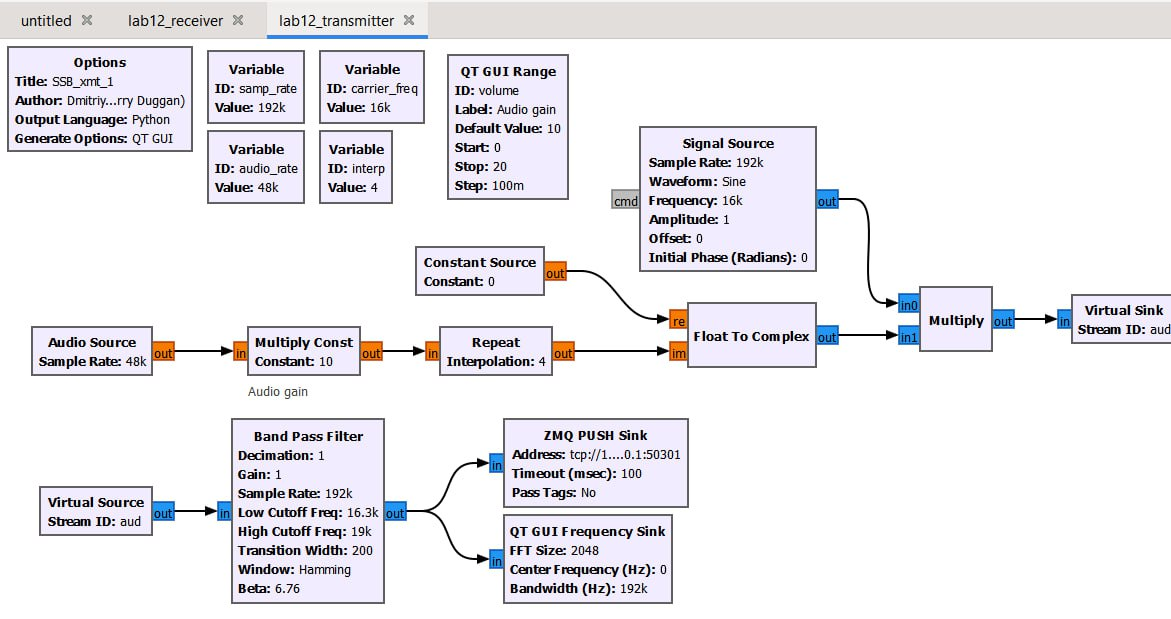
\includegraphics[width=\textwidth]{ssb_transmitter_flowgraph.jpg}
\caption{SSB transmitter flowgraph}
\end{figure}

\section{Тестирование}

Для тестирования полученной системы воспользуемся двумя терминалами для параллельного запуска примемника и передатчика.\\

В первом терминале запустим приемник командой: \texttt{python -u lab12\_receiver.py}. Увидим открывшийся интерфейс GUI со слайдерами для регулировки параметров.\\

Во втором терминале выполним \texttt{python -u lab12\_transmitter.py} и откроется второе окно с регулировкой усиления звука и стоком частоты.\\
\vspace{1cm}

\begin{figure}[H]
\centering
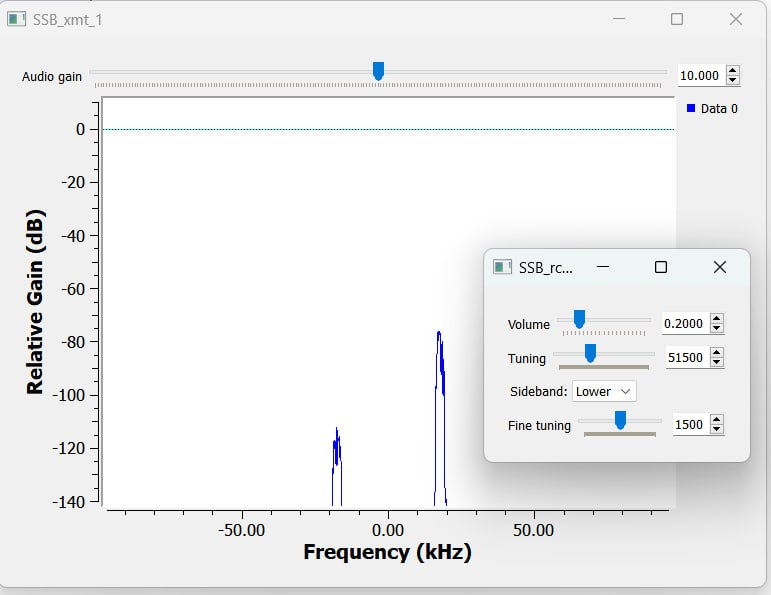
\includegraphics[width=\textwidth]{ssb_test}
\caption{Отображение частот модуляции}
\end{figure}

Подача звука в микрофон выдает изменения в паттерне QT GUI Time Sink. Уровень модуляции сопоставим с transmit gain control. На динамиках слышен голос.

\section*{Вывод}
\addcontentsline{toc}{section}{\protect\numberline{}Вывод}
В ходе выполнения лабораторной работы было произведено знакомство с GNU Radio, интерфейсом GRC а также с однополосным приемо-передатчиком.

\end{document}



